\documentclass{article}
\usepackage[utf8]{inputenc}
\usepackage{graphicx}
\usepackage{amsmath}
\usepackage{geometry}
\geometry{a4paper}

\title{Análisis de Escenas 2D con Operaciones Vectoriales}
\author{Nombre del Estudiante: alexdith ariza - nelson martinez\\
        Curso: Simulacion y robotica \\
        Profesor: jorge rudas}
\date{\ 03/03/2025}

\begin{document}

\maketitle

\begin{abstract}
Este informe presenta el análisis y representación de escenas 2D mediante operaciones vectoriales. Utilizando Python y la librería `matplotlib`, se generan diferentes escenas que incluyen un fondo rectangular y un punto. Se implementaron operaciones de desplazamiento y rotación del punto en un sistema 2D utilizando álgebra vectorial. Las gráficas generadas reflejan los efectos de estas operaciones, y se proporciona un análisis detallado de los resultados obtenidos.
\end{abstract}

\section{Introducción}
En este trabajo, se realiza el estudio y la representación de escenas 2D utilizando operaciones vectoriales para manipular las posiciones de puntos sobre un fondo rectangular. Se aborda el uso de la librería `matplotlib` en Python para visualizar las escenas y las transformaciones que se aplican a los puntos mediante desplazamientos y rotaciones.

El propósito principal es entender cómo las operaciones vectoriales pueden modelar y transformar objetos en un espacio 2D. Estas operaciones se aplican en un contexto visual, lo que permite obtener una comprensión clara y práctica de la manipulación de puntos en gráficos computacionales.

\section{Objetivos de la Actividad}
Los objetivos de esta actividad son:
\begin{itemize}
    \item Representar escenas 2D utilizando un fondo rectangular y puntos superpuestos.
    \item Realizar operaciones vectoriales sobre los puntos, como desplazamiento y rotación.
    \item Visualizar los efectos de las operaciones vectoriales en las escenas generadas.
    \item Analizar los resultados mediante gráficas y proporcionar una interpretación detallada de las transformaciones.
\end{itemize}

\section{Descripción de la Actividad y/o Documentación de Código}
Para cumplir con los objetivos, se implementó una clase `Escena` en Python. La clase permite definir una escena con un fondo rectangular y un punto, realizando operaciones sobre este punto utilizando álgebra vectorial. Las funciones clave implementadas en el código son:
\begin{itemize}
    \item \texttt{mostrar()}: Muestra la escena con el fondo y el punto.
    \item \texttt{desplazar\_punto()}: Desplaza el punto usando un vector de desplazamiento.
    \item \texttt{rotar\_punto()}: Rota el punto alrededor del origen usando una matriz de rotación 2D.
\end{itemize}

El código utiliza la librería `matplotlib` para la visualización gráfica de las escenas y las transformaciones realizadas sobre los puntos.

\section{Gráficas de Resultados}
A continuación, se presentan las gráficas de las tres escenas generadas:

\begin{figure}[h!]
    \centering
    \includegraphics[width=0.7\textwidth]{escena1.png}
    \caption{Primera escena: Fondo verde claro y punto morado.}
    \label{fig:escena1}
\end{figure}

\begin{figure}[h!]
    \centering
    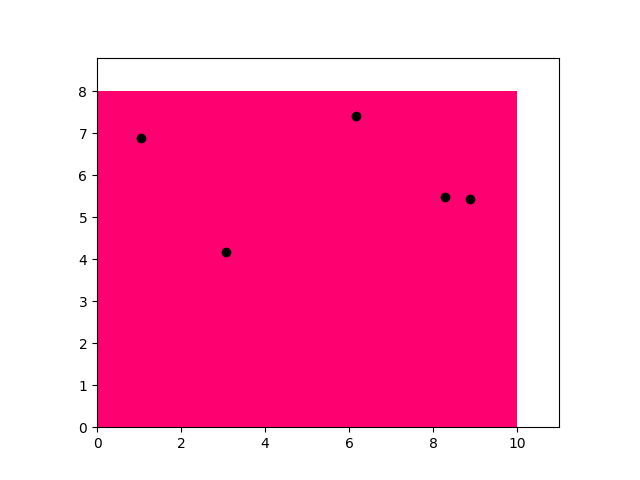
\includegraphics[width=0.7\textwidth]{escena2.png}
    \caption{Segunda escena: Fondo azul cielo y punto naranja.}
    \label{fig:escena2}
\end{figure}

\begin{figure}[h!]
    \centering
    \includegraphics[width=0.7\textwidth]{escena3.png}
    \caption{Tercera escena: Fondo amarillo y punto negro.}
    \label{fig:escena3}
\end{figure}

\section{Análisis de las Gráficas}
Cada una de las gráficas muestra una escena con un fondo rectangular y un punto en diferentes posiciones. A continuación se detalla el análisis de cada una:

\subsection{Primera Escena}
La primera escena tiene un fondo de color verde claro y un punto morado en la posición \((5,5)\). El desplazamiento del punto se realiza por un vector de \([2, 3]\), lo que mueve el punto a la posición \((7,8)\). La gráfica muestra claramente el punto desplazado.

\subsection{Segunda Escena}
La segunda escena tiene un fondo de color azul cielo con un punto naranja ubicado inicialmente en la posición \((3, 7)\). Se realiza una rotación del punto 45 grados. La gráfica muestra cómo el punto cambia de posición después de la rotación, lo que evidencia el efecto de la operación vectorial de rotación.

\subsection{Tercera Escena}
La tercera escena tiene un fondo amarillo y un punto negro ubicado en la posición \((2, 2)\). Se realiza un desplazamiento del punto por el vector \([-1, -1]\), lo que mueve el punto a la nueva posición \((1, 1)\). La gráfica muestra claramente el resultado del desplazamiento.

\section{Interpretación de los Resultados}
Los resultados muestran cómo las operaciones vectoriales afectan la posición del punto en el espacio 2D:
\begin{itemize}
    \item El desplazamiento traslada el punto en una dirección específica definida por el vector de desplazamiento.
    \item La rotación cambia la dirección del punto respecto al origen, manteniendo su distancia, pero alterando su orientación.
\end{itemize}

Las gráficas proporcionan una visualización clara de estos efectos, ayudando a comprender cómo las transformaciones geométricas afectan a los objetos en un plano.

\section{Conclusiones}
A través de esta actividad, hemos aprendido a aplicar operaciones vectoriales para manipular y visualizar puntos en un sistema 2D. Las transformaciones de desplazamiento y rotación son fundamentales para el modelado de escenas en gráficos computacionales. Además, la visualización de los efectos de estas operaciones permite una mejor comprensión de cómo se manipulan los objetos en el espacio. Este enfoque es esencial para el análisis y diseño de sistemas gráficos y simulaciones visuales.

\end{document}
